\documentclass[xcolor=dvipsnames]{beamer}

\usepackage{graphicx}
\usepackage{listings}
\usepackage{comment}
\usepackage{float}
\usepackage{tikz}
\usepackage{algorithm}
\usepackage[noend]{algorithmic}

\usetikzlibrary{arrows}

\usetheme{Frankfurt}
%\usecolortheme[named=OliveGreen]{structure}
%\usefonttheme{serif}
\setbeamertemplate{navigation symbols}{}
\setbeamertemplate{frametitle}[default][center]

\newcommand{\ReadArrowType}{latex}

\newcommand{\BidirectedEdgeForward}[2]{
		\tikz[>=triangle 45,baseline]
		\draw[>->,thin] (0,0.1) node[anchor=east] {#1} --
					    (0.8,0.1) node[anchor=west] {#2};}

\newcommand{\LengthVar}{L}

\begin{document}
\title{A Bidirected String Graph Model of Genome Assembly}
\author{Eric Biggers}
\institute{Macalester College}
\date{December 5, 2012}
%\titlegraphic{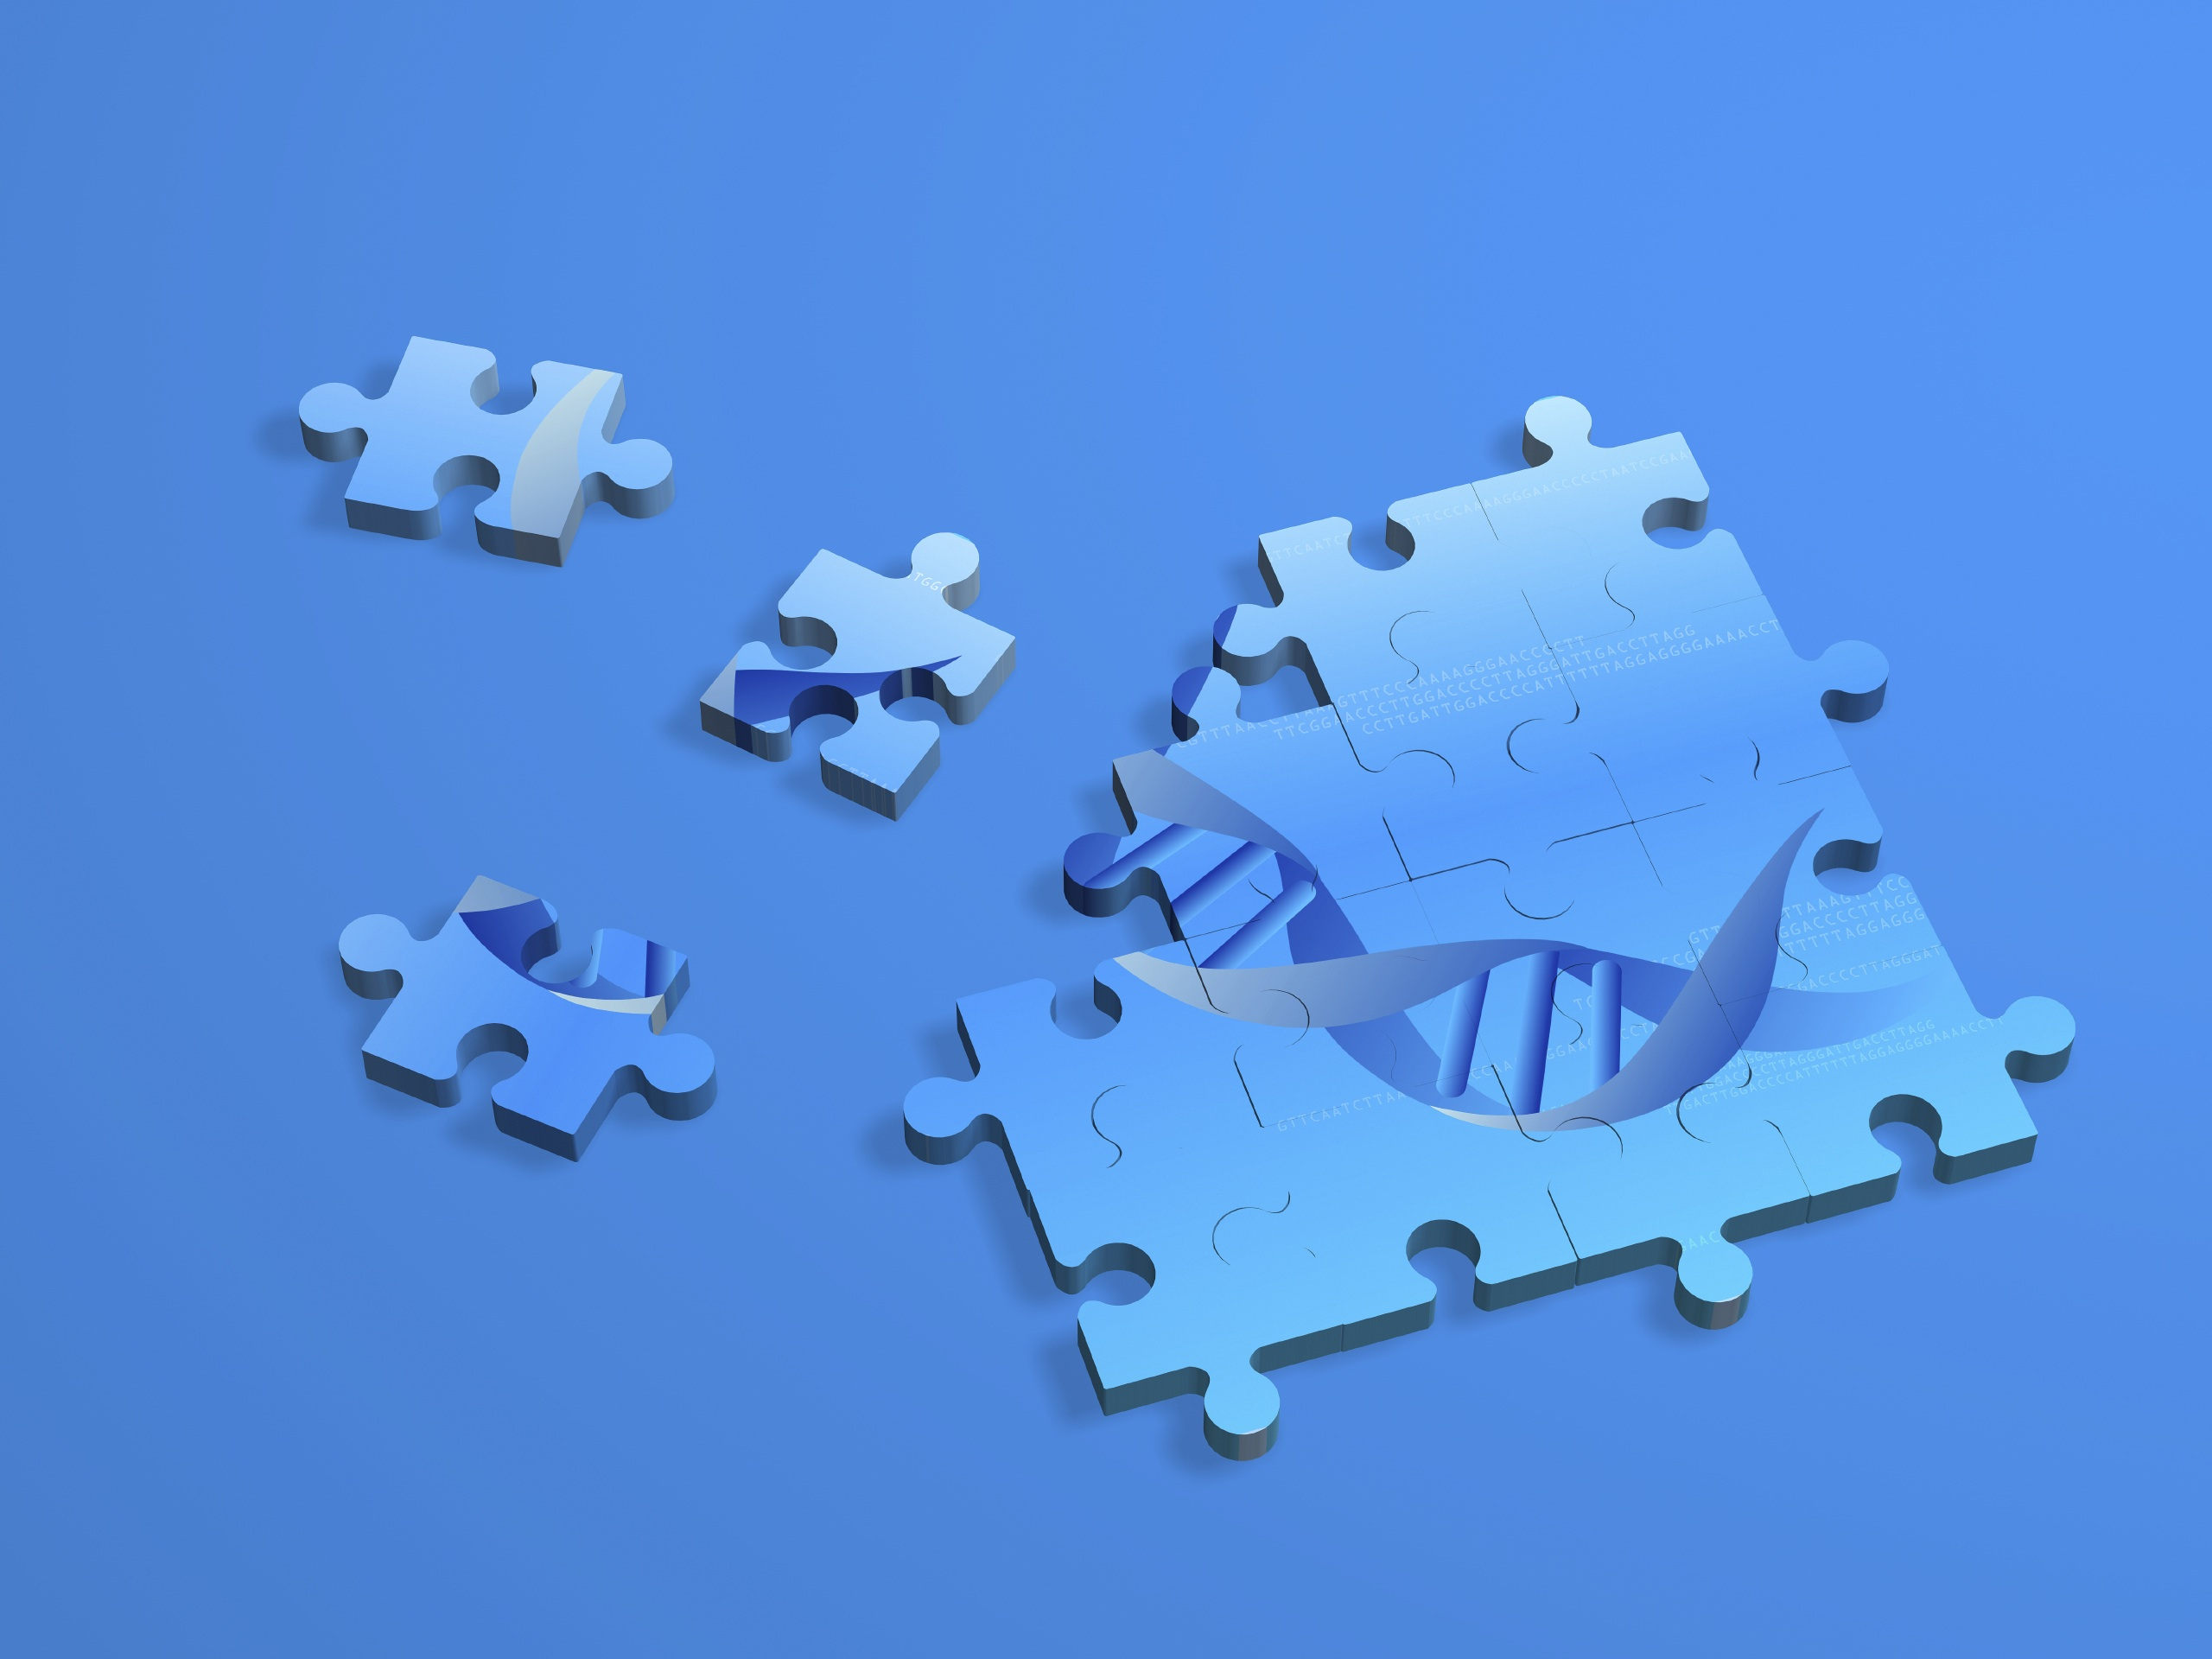
\includegraphics[width=\textwidth,clip=true,trim=0 300 0 500]{puzzle.jpg}}


\frame{\titlepage}

\begin{frame}{Genomes}
	\begin{itemize}
		\item A genome (for our purposes) is a long string of A's, C's, G's, and T's
		\item Genomes are dual-stranded
		\begin{itemize}
			\item {\tt A} always pairs with {\tt T} and {\tt C} always pairs
			with {\tt G}
			\item The two strands run in opposite directions
		\end{itemize}
	\end{itemize}
	\begin{center}
	{\tt $\leftarrow$ GTTGCTATAAATACGGGTCATGGTATTTTAGTACCG $\leftarrow$ \\}
	{\tt $\rightarrow$ CAACGATATTTATGCCCAGTACCATAAAATCATGGC $\rightarrow$}
	\end{center}
	\begin{itemize}
		\item Each letter in the genome is called a {\bf base pair} \\(abbreviation:
		{\bf bp})
	\end{itemize}
	\begin{table}[H]
		\caption{Approximate genome sizes of selected organisms}
		\begin{tabular}{|c|c|c|}
			\hline
			{\it E. coli} (a bacterium) &  ~4,600,000 bp \\
			\hline
			{\it Ananas comosus} (pineapple plant) &	~500,000,000 bp \\
			\hline
			{\it Homo sapiens} (human)       &  ~3,000,000,000 bp \\
			\hline
		\end{tabular}
	\end{table}
\end{frame}

\begin{frame}{Genome Sequencing}
	\begin{itemize}
		\item How can we determine the precise base-pair sequence of an
		organism's genome?

		\item Currently available sequencing technologies can only sequence
		fragments a few dozen to a few thousand bp long

		\item Genome assembly:
			\begin{itemize}
				\item Lab work
				\begin{enumerate}[1.]
						\item Obtain a DNA sample
						\item Break DNA into much smaller fragments
						\item Sequence the fragments using available technology
				\end{enumerate}
				\item Computational Work
				\begin{enumerate}[4.]
					\item Given the sequenced fragments, reconstruct the original genome.
				\end{enumerate}
			\end{itemize}
	\end{itemize}
\end{frame}

\begin{frame}{Reads}
	\begin{itemize}
		\item A {\bf read} is a short sequence of base pairs that represents
		some DNA that was sequenced by the sequencing machine.
		\item A read may come from any location on the genome, from either
		strand.
		\item Reads from opposite strands go in opposite directions.
			\begin{itemize}
				\item As a result, a sequence and its {\bf reverse-complement}
				(the corresponding sequence on the other strand, going
				backwards) are usually considered equivalent.
			\end{itemize}
	\end{itemize}
		{\scriptsize
			{\tt 1.}
			\hspace*{-0.03cm}{\tt\color{red}$\leftarrow$TGAGCTTAAGGCTTATCTATCTTCAGACGACA$\leftarrow$ }\\
			{\tt 2.}
			\hspace*{1.76cm}{\tt \color{red} $\leftarrow$TTATCTATCTTCAGACGACTATTATAGCGCGG$\leftarrow$}\\
			{\tt G.}
			{\tt $\leftarrow$TGAGCTTAAGGCTTATCTATCTTCAGACGACTATTATAGCGCGGCCAAGACTACGCGGAGCCCC$\leftarrow$} \\
			{\tt G.}
			{\tt $\rightarrow$ACTCGAATTCCGAATAGATAGAAGTCTGCTGATAATATCGCGCCGGTTCTGATGCGCCTCGGGG$\rightarrow$} \\
			{\tt 3.} \hspace*{3.55cm}{\tt \color{blue} $\rightarrow$TCTGCTGATAATATCGCGCCGGTTCTGATGCG$\rightarrow$}
			\vspace{0.5cm}
		}
		\\
		{\footnotesize Above: a very short genome (G.) and three reads that came from it (1.,
		2., 3.).}
\end{frame}


\begin{frame}{Genome assemblers}
	\begin{itemize}
		\item An {\bf assembler} is a program or algorithm that can put together
		a set of reads to reconstruct the original genome.  (Think of putting
		together a puzzle $\dots$)
		\item  Input: a set of reads (lengths: ~35 to 5000bp each).
		\item  Output: one strand of the reconstructed genome (if possible)--- but
		in general, an exact answer may be impossible, so the actual output is a
		set of substrings of the original genome that are as long as possible.
		(lengths: ~10,000 to 10,000,000bp each).
	\end{itemize}
\end{frame}

\begin{frame}[fragile]{Details of assembler input}
	\begin{itemize}
		\item The reads given to an assembler (my code, as well as most
		other assemblers) as input can be in a simple plain-text format:
	\end{itemize}
	\begin{verbatim}
	>read_1
	AAATCGGCGCGTAAACAGGCAGCCAGCACCGCAGCA
	>read_2
	GAGTAGTCGGAACCGTTGCGTCCAAGCATTAGTGTA
	>read_3
	TAGCGGCCAGGATGCTTTACCCAATATCAGCGATGC
	...
	\end{verbatim}
	\begin{itemize}
		\item The assembler may use other DNA sequence representations
		(e.g. a binary representation with 2 bits per base) internally.
	\end{itemize}
\end{frame}

\begin{frame}[fragile]{Details of assembler output}
	\begin{itemize}
		\item Most assemblers can generate output in the same plain-text
		format.
		\item A {\bf contig} is a continuous sequence of DNA that was
		assembled.  Ideally, each contig should be much longer than the
		original reads.
	\end{itemize}
	\begin{verbatim}
	>contig_1
	GTTGCGAGATTTGGACGGACGTTGACGGGGTCTATACCTGCGACCCGCGTCA
	GGTGCCCGATGCGAGGTTGTTGAAGTCGATGTCCTACCAGGAAGCGATGGAG
	CTTTCCTACTTCGGCGCTAAAGTTCTTCACCCCCGCACCATTACCCCCATCG
	CCCAGTTCCAGATCCCTTGCCTGATTAAAAATACCGGAAATCCTCAAGCACC
	AGGTACGCTCATTGGTGCCAGCCGTGATGAAGACGAATTACCGGTCAAGGGC
	ATTTCCAATCTGAATAACATGGCAATGTTCAGCGTTTCTGGTCCGGGGATGA
	...
	\end{verbatim}
\end{frame}

\begin{frame}{Genome assembly vs Shortest Common Substring}
	Genome assembly is superficially similar to the shortest common superstring
	(SCS) problem, which is to find the shortest string that contains all strings
	from a given set.
	\begin{center}
	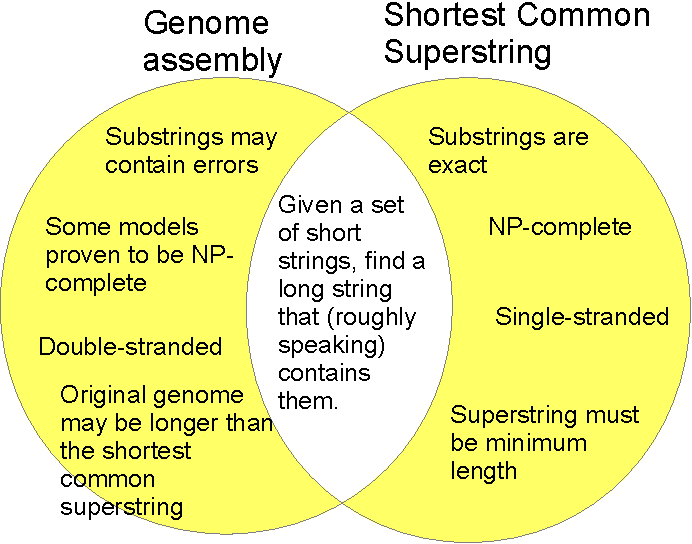
\includegraphics[scale=0.6]{venn-crop.pdf}
	\end{center}
\end{frame}

\begin{frame}{An algorithm for genome assembly}

	\begin{itemize}
		\item {\it The fragment string assembly graph} (Myers, 2005)
		\item Draws on ideas used in previous assemblers and also introduces new
		ideas
		\item The fundamental algorithm:
		\begin{enumerate}
			\item Use overlaps between reads to build a graph that models the
			assembly problem.
			\item Simplify and analyze the graph.
			\item Find paths through the graph to reconstruct the original
			sequence.
		\end{enumerate}
	\end{itemize}
\end{frame}

\begin{frame}{Overlaps between reads}
	Consider two reads, $f$ and $g$, and their reverse-complements $f'$ and $g'$.
	The reads $f$ and $g$ are said to {\bf exactly overlap} by some length
	$\LengthVar$ iff at least one of the following is true:
	\begin{itemize}
		\item The last $\LengthVar$ bp of $f$ exactly match the first
		$\LengthVar$ bp of $g$.
		\item The last $\LengthVar$ bp of $f$ exactly match the first
		$\LengthVar$ bp of $g'$.
		\item The last $\LengthVar$ bp of $f'$ exactly match the first
		$\LengthVar$ bp of $g$.
		\item The last $\LengthVar$ bp of $f'$ exactly match the first
		$\LengthVar$ bp of $g'$.
	\end{itemize}
	An exact overlap $o$ is fully described by the tuple $(f, g, f_{beg},
	g_{beg}, len, rc)$.
	%there $f$ and $g$ are the reads of the overlap,
	%$f_{beg}$ and $g_{beg}$ and the starting position of the overlap on each
	%read, $len$ is the length of the overlap, and $rc$ indicates whether the
	%overlap is reverse-complement or not.
\end{frame}

\begin{frame}{Overlaps between reads}

	\begin{itemize}
	\item Two reads that overlap are likely to come from adjacent positions on the genome.
	\end{itemize}

	{\tt Read 1: \ \ \ \ \ \ \ \ \ $\rightarrow$
		ATATAT\textcolor{red}{GCTGGTTACTT} $\rightarrow$ } \\
	{\tt Read 2: \ \ \ \ \ \ \ \ \ \ \ \ \ \ \ $\rightarrow$
		\textcolor{red}{GCTGGTTACTT}TGATAGATA $\rightarrow$ } \\
	{\tt Possible genome: $\rightarrow$ ATATATGCTGGTTACTTTGATAGATA $\rightarrow$}

	\begin{itemize}
	\item Overlapping reads may be from different strands, in which case the
	overlapped regions are reverse-complement from each other.
	\end{itemize}

	{\tt Read 1: \ \ \ \ \ \ \ \ \ $\rightarrow$
		ATATAT\textcolor{red}{GCTGGTTACTT} $\rightarrow$ } \\
	{\tt Read 2: \ \ \ \ \ \ \ \ \ \ \ \ \ \ \ $\leftarrow$
		\textcolor{red}{CGACCAATGAA}ACTATCTAT $\leftarrow$ } \\
	{\tt Possible genome: $\rightarrow$ ATATATGCTGGTTACTTTGATAGATA $\rightarrow$}
\end{frame}

\begin{frame}{Three types of overlaps}
	\begin{enumerate}
		\item ``Normal'' overlap
			\begin{center}
				\vspace{-0.5cm}
				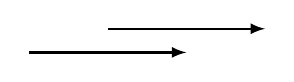
\begin{tikzpicture}[>=\ReadArrowType]
					\draw[->,style=thick] (0,0) -- (2,0);
					\draw[->,style=thick] (1.0,0.3) -- (3.0,0.3);
				\end{tikzpicture}

				\vspace{3mm}
				or (symmetrically)
				\vspace{3mm}

				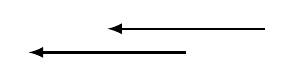
\begin{tikzpicture}[>=\ReadArrowType]
					\draw[->,style=thick] (2,0) -- (0,0);
					\draw[->,style=thick] (3.0,0.3) -- (1.0,0.3);
				\end{tikzpicture}
			\end{center}
		\vspace{0.5cm}
		\item ``Innie'' overlap
			\begin{center}
				\vspace{-0.5cm}
				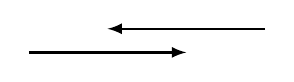
\begin{tikzpicture}[>=\ReadArrowType]
					\draw[->,style=thick] (0,0) -- (2,0);
					\draw[->,style=thick] (3,0.3) -- (1,0.3);
			\end{tikzpicture} \end{center}
		\vspace{0.5cm}
		\item ``Outie'' overlap
			\begin{center}
			\vspace{-0.5cm}
			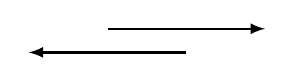
\begin{tikzpicture}[>=\ReadArrowType]
					\draw[->,style=thick] (2,0) -- (0,0);
					\draw[->,style=thick] (1.0,0.3) -- (3.0,0.3);
			\end{tikzpicture} \end{center}
	\end{enumerate}
\end{frame}


\begin{frame}{Computing overlaps}
	\begin{itemize}
		\item Goal: compute all pairwise overlaps of some minimum length
		$\LengthVar$ among the reads.
		\item Naive algorithm compares every read with every other read ($N$
		reads: $N^2$ time)
		\item A faster algorithm indexes the reads by short subsequences, then
		only compares reads that share a subsequence
		(``seed-and-extend'').
		\item Overlaps may be exact, or they may allow for differences up to a
		certain threshold.
	\end{itemize}
\end{frame}

\begin{frame}{Computing overlaps (Implementation)}
	\begin{itemize}
		\item Implementation: {\tt compute-overlaps}
			\begin{itemize}
				\item {\bf Input}:  A set of reads and the minimum overlap
				length $\LengthVar$
				\item {\bf Output}:  All exact pairwise overlaps between reads,
				including reverse-complement overlaps
				\item {\bf Algorithm}:  Seed-and-extend
				\item {\bf Running time}: Linear with respect to genome length
				for non-repetitive genomes; quadratic with respect to read
					density; quadratic with respect to the number of times a
					sequence of DNA is repeated in the genome
			\end{itemize}
	\end{itemize}
	%\begin{algorithm}[H]
		%\caption{Algorithm {\sc compute-overlaps}($S$)}
		%\begin{algorithmic}
			%%\STATE{h = new hash table}
			%%\FOR{{\bf each} read $r \in S$}
				%%\FOR{{\bf each} canonical $k$-mer $K \in R$}
					%%\STATE{Append $K.pos$ to $h[K]$}
				%%\ENDFOR
			%%\ENDFOR
			%%\FORALL{posList $\in h$}
				%%\FORALL{$k$-mer pairs $k1$, $k2$ in
			%%\ENDFOR
		%\end{algorithmic}
	%\end{algorithm}
\end{frame}

\begin{frame}{Build the fragment string assembly graph}
	\begin{itemize}

		\item Use the overlaps to construct a graph modeling how the reads could
		be put together
		\item Make each read be a vertex
		\item Make each edge be an overlap
		\begin{itemize}
			\item Two reads are connected with an edge iff they share an overlap.
		\end{itemize}
		\item Label each edge with an appropriate DNA sequence; this makes the
		graph a {\bf string graph}.
		\item Should the edges be directed or undirected?  \\Or $\dots$ something
		else?
	\end{itemize}
\end{frame}

\begin{frame}{Build the fragment string assembly graph (cont.)}
	\begin{itemize}
		\item At this stage, we don't know which strands the reads are from!

		\begin{center}
			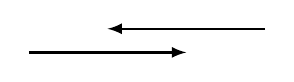
\begin{tikzpicture}[>=\ReadArrowType]
				\draw[->,style=thick] (0,0) -- (2,0);
				\draw[->,style=thick] (3,0.3) -- (1,0.3);
			\end{tikzpicture}
			\hspace{5mm}or\hspace{5mm}
			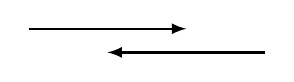
\begin{tikzpicture}[>=\ReadArrowType]
				\draw[->,style=thick] (0,0.3) -- (2,0.3);
				\draw[->,style=thick] (3, 0) -- (1, 0);
			\end{tikzpicture}
			\hspace{5mm} ?
		\end{center}

		\item We must allow each read to be used either in the
		reverse-complement or forward direction.
		\item Therefore, we must allow the edges to be traversed in either
		direction.
		\item However, each read must still be used in a consistent way within
		any single assembly.
		\item Solution: use a {\bf bidirected graph}.
	\end{itemize}
\end{frame}

\begin{frame}{Bidirected Graphs}
	\begin{itemize}
		\item A {\bf bidirected graph} is a graph where a directed head is
		attached to both ends of each edge.

		\item There are 3 (or 4, ignoring symmetry) types of {\bf bidirected
		edges}.  They follow directly from the different types of overlaps.

		\begin{center}
			\begin{tabular}{p{1cm}cccc}
				{\footnotesize Overlap} &
				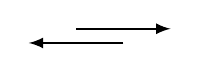
\begin{tikzpicture}[scale=0.6,>=\ReadArrowType]
						\draw[->,style=thick] (2,0) -- (0,0);
						\draw[->,style=thick] (1,0.3) -- (3,0.3);
				\end{tikzpicture}
				&
				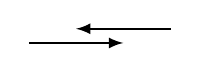
\begin{tikzpicture}[scale=0.6,>=\ReadArrowType]
						\draw[->,style=thick] (0,0) -- (2,0);
						\draw[->,style=thick] (3,0.3) -- (1,0.3);
				\end{tikzpicture}
				&
				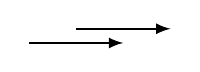
\begin{tikzpicture}[scale=0.6,>=\ReadArrowType]
						\draw[->,style=thick] (0,0) -- (2,0);
						\draw[->,style=thick] (1,0.3) -- (3,0.3);
				\end{tikzpicture}
				&
				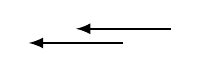
\begin{tikzpicture}[scale=0.6,>=\ReadArrowType]
						\draw[->,style=thick] (2,0) -- (0,0);
						\draw[->,style=thick] (3,0.3) -- (1,0.3);
				\end{tikzpicture}
				\\
				&$\downarrow$ & $\downarrow$& $\downarrow$& $\downarrow$ \\
				{\footnotesize Bidirected edge} &
				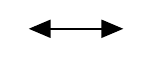
\begin{tikzpicture}[scale=0.6,>=triangle 45]
						\draw[<->,style=thick] (0,0) -- (2,0);
				\end{tikzpicture}
				&
				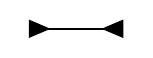
\begin{tikzpicture}[scale=0.6,>=triangle 45]
						\draw[>-<,style=thick] (0,0) -- (2,0);
				\end{tikzpicture}
				&
				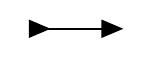
\begin{tikzpicture}[scale=0.6,>=triangle 45]
						\draw[>->,style=thick] (0,0) -- (2,0);
				\end{tikzpicture}
				&
				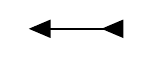
\begin{tikzpicture}[scale=0.6,>=triangle 45]
						\draw[<-<,style=thick] (0,0) -- (2,0);
				\end{tikzpicture}
			\end{tabular}
		\end{center}

		%\item Two vertices (reads) may have multiple {\bf bidirected edges}
		%between them if they overlap in different ways, but there can be at most
		%one bidirected edge {\em of the same type} between two vertices if we
		%always prefer the best overlap of a given type.
	\end{itemize}
\end{frame}

\begin{frame}{Walks in a bidirected graph}
	\begin{itemize}
		\item A {\bf walk in a bidirected graph} $G$ is a continuous sequence of
		edges in $G$ such that if any vertex $v$ is entered through a head
		inwards, it is left on a head outwards (unless it is the end of the
		path), and vice versa.
		\item A bidirected edge may be traversed in opposite directions during
		the same walk.
		\item The reverse of a walk in a bidirected graph is also a
		valid walk.
		\item $1 \to 2 \to 3 \to 4$ and $4 \to 3 \to 2 \to 1$ are both valid
		walks in the bidirected graph below.
	\end{itemize}
		\begin{center} {\small
		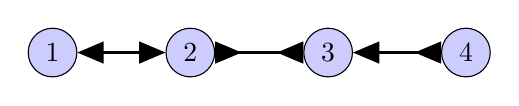
\begin{tikzpicture}[>=triangle 45]
			\tikzstyle{every node} = [circle,fill=blue!20,draw=black];
			\node (1) at (0.00, 0) {1};
			\node (2) at (1.75, 0) {2};
			\node (3) at (3.50, 0) {3};
			\node (4) at (5.25, 0) {4};
			\draw[<->,very thick] (1) edge (2);
			\draw[>-<,very thick] (2) edge (3);
			\draw[<-<,very thick] (3) edge (4);
		\end{tikzpicture} } \end{center}
\end{frame}

\begin{frame}{Walking through the bidirected string graph}
	\begin{itemize}
		\item A walk through a bidirected string graph constructed from read
		overlaps models a way in which the reads can be assembled together
		consistently.

		\item Each read may be used in forward or reverse-complement
		orientation, depending on the orientation of the arrow head when the
		corresponding vertex is entered.
	\end{itemize}
	\begin{figure}[H]
		{\small
		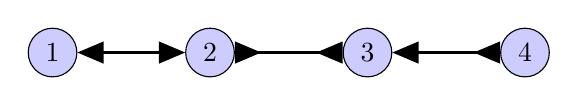
\begin{tikzpicture}[>=triangle 45]
			\tikzstyle{every node} = [circle,fill=blue!20,draw=black];
			\node (1) at (0.00, 0) {1};
			\node (2) at (2.0, 0) {2};
			\node (3) at (4.0, 0) {3};
			\node (4) at (6.0, 0) {4};
			\draw[<->,very thick] (1) edge (2);
			\draw[>-<,very thick] (2) edge (3);
			\draw[<-<,very thick] (3) edge (4);
		\end{tikzpicture} }

		\vspace{2.5mm}

		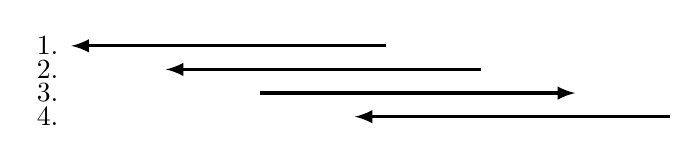
\begin{tikzpicture}[>=\ReadArrowType]
				\draw[<-,style=very thick] (0.0, 0.0) -- (4.0, 0.0);
				\draw[<-,style=very thick] (1.2, -0.3) -- (5.2, -0.3);
				\draw[->,style=very thick] (2.4, -0.6) -- (6.4, -0.6);
				\draw[<-,style=very thick] (3.6, -0.9) -- (7.6, -0.9);
				\draw (-0.3, 0.0) node {1.};
				\draw (-0.3, -0.3) node {2.};
				\draw (-0.3, -0.6) node {3.};
				\draw (-0.3, -0.9) node {4.};
		\end{tikzpicture}
		\caption{A bidirected graph and the implied assembly of the
		corresponding reads}
	\end{figure}
\end{frame}


\begin{frame}{Transitive reduction}
	\begin{itemize}
		\item Very commonly, given three adjacent reads $f$, $g$, and $h$, $f$
		will overlap $h$ as well as $g$.  This is redundant because we can,
		equivalently, walk $f$ to $g$ to $h$ rather than directly walking from
		$f$ to $h$.

		\begin{center}
			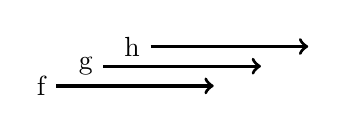
\begin{tikzpicture}
				\draw[->,style=very thick] (0,0) node[anchor=east] {f} -- (2,0);
				\draw[->,style=very thick] (0.6,0.25) node[anchor=east] {g} -- (2.6,0.25);
				\draw[->,style=very thick] (1.2,0.5) node[anchor=east] {h} -- (3.2,0.5);
			\end{tikzpicture}
			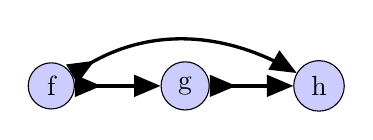
\begin{tikzpicture}[>=triangle 45]
				\tikzstyle{every node} = [circle,fill=blue!20,draw=black];
				\node (f) at (0, 0) {f};
				\node (g) at (1.7, 0) {g};
				\node (h) at (3.4, 0) {h};
				\draw[>->,style=very thick] (f) edge (g);
				\draw[>->,style=very thick] (g) edge (h);
				\draw[>->,style=very thick,bend left] (f) edge (h);
			\end{tikzpicture}
		\end{center}

		\item Walks visiting more vertices are preferred because they are
		supported by more reads and the overlaps tend to be longer.  So, we
		would like to throw away \BidirectedEdgeForward{$f$}{$h$} but keep
		\BidirectedEdgeForward{$f$}{$g$} and \BidirectedEdgeForward{$g$}{$h$}.

		\item To remove these redundant edges, {\bf transitive reduction} is
		performed on the bidirected string graph.
	\end{itemize}
\end{frame}

\begin{frame}{Transitive reduction (cont.)}
		Transitive reduction algorithm:  Go through each vertex $v$ and
		examine vertices up to 2 edges away from $v$ to identify all
		transitive edges leaving $v$.
	\begin{algorithm}[H]
		\caption{{\sc TransitiveReduction}($G$)}
	{\footnotesize
		\begin{algorithmic}
			\FOR{{\bf each} vertex $v \in G$}
				\STATE{Mark all neighbors of $v$ as {\tt INPLAY}}
				\STATE{Set {\tt longest} $\gets$ length of the longest edge leaving $v$}
				\FOR{{\bf each} edge $v \to w$ in order of length}
					\FOR{{\bf each} edge $w \to x$ in order of length}
						\IF{$x$ is not marked {\tt INPLAY}}
							\STATE{\bf continue}
						\ENDIF
						\IF{$len(v \to w) + len(w \to x) > $ {\tt longest}}
							\STATE{\bf break}
						\ENDIF
						\STATE{Mark $x$ as {\tt ELIMINATED}}
					\ENDFOR
				\ENDFOR
				\STATE{Mark as transitive all edges $v \to x$ where $x$ is marked {\tt ELIMINATED}}
			\ENDFOR
			\STATE{Eliminate all edges marked transitive}
		\end{algorithmic}
	}
	\end{algorithm}
\end{frame}

\begin{frame}{Collapsing unbranched paths}

Vertex 4 below is an {\bf inner vertex} that is part of an unbranched path that
can be collapsed.

\begin{center}
	{\small
	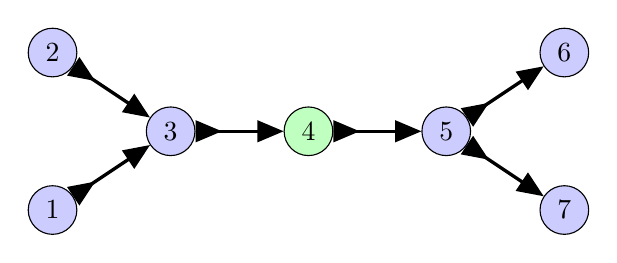
\begin{tikzpicture}[>=triangle 45]
		\tikzstyle{every node} = [circle,fill=blue!20,draw=black];
		\node (1) at (0.0, -1) {1};
		\node (2) at (0.0, 1) {2};
		\node (3) at (1.5, 0) {3};
		\node[fill=green!25] (4) at (3.25, 0) {4};
		\node (5) at (5.0, 0) {5};
		\node (6) at (6.5, 1) {6};
		\node (7) at (6.5, -1) {7};
		\draw[>->,very thick] (1) edge (3);
		\draw[>->,very thick] (2) edge (3);
		\draw[>->,very thick] (3) edge (4);
		\draw[>->,very thick] (4) edge (5);
		\draw[>->,very thick] (5) edge (6);
		\draw[>->,very thick] (5) edge (7);
	\end{tikzpicture}
	}

becomes:

	{\small
	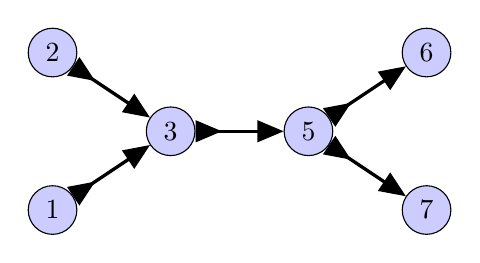
\begin{tikzpicture}[>=triangle 45]
		\tikzstyle{every node} = [circle,fill=blue!20,draw=black];
		\node (1) at (0.0, -1) {1};
		\node (2) at (0.0, 1) {2};
		\node (3) at (1.5, 0) {3};
		\node (5) at (3.25, 0) {5};
		\node (6) at (4.75, 1) {6};
		\node (7) at (4.75, -1) {7};
		\draw[>->,very thick] (1) edge (3);
		\draw[>->,very thick] (2) edge (3);
		\draw[>->,very thick] (3) edge (5);
		\draw[>->,very thick] (5) edge (6);
		\draw[>->,very thick] (5) edge (7);
	\end{tikzpicture}
	}
\end{center}
\end{frame}

\begin{frame}{Current state of the graph}
	\begin{itemize}
		\item Non-repetitive genomes and/or long reads: The assembly is already
		complete!
	\end{itemize}

	\vspace{1cm}

	\begin{figure}[H]
		\begin{tikzpicture}
			{\small
			\begin{tikzpicture}[>=triangle 45]
				\node[circle,fill=blue!20,draw=black] (A) at (0.0, 0) {A};
				\node[circle,fill=blue!20,draw=black] (B) at (3.0, 0) {B};
				\draw[>->,very thick] (A) edge node[anchor=north] {4639100} (B);
			\end{tikzpicture} }
		\end{tikzpicture}
		\caption{
			Bidirected string graph for reads uniformly sampled from a 4.6 Mbp
			random genome after transitive reduction and path collapsing.  (Edge
			labeled with length of sequence)}
	\end{figure}
\end{frame}

\begin{frame}{Current state of the graph (cont.)}
	\begin{itemize}
		\item Repetitive genomes and/or short reads: The graph will still be
		very complicated.
		\item Swap out the 4.6 Mbp random genome with {\it E. coli}'s genome,
		which is the same size but contains some repeats, and we get a
		complicated graph, {\bf even after increasing the read length to
		1000bp}:
	\end{itemize}
	\begin{center}
		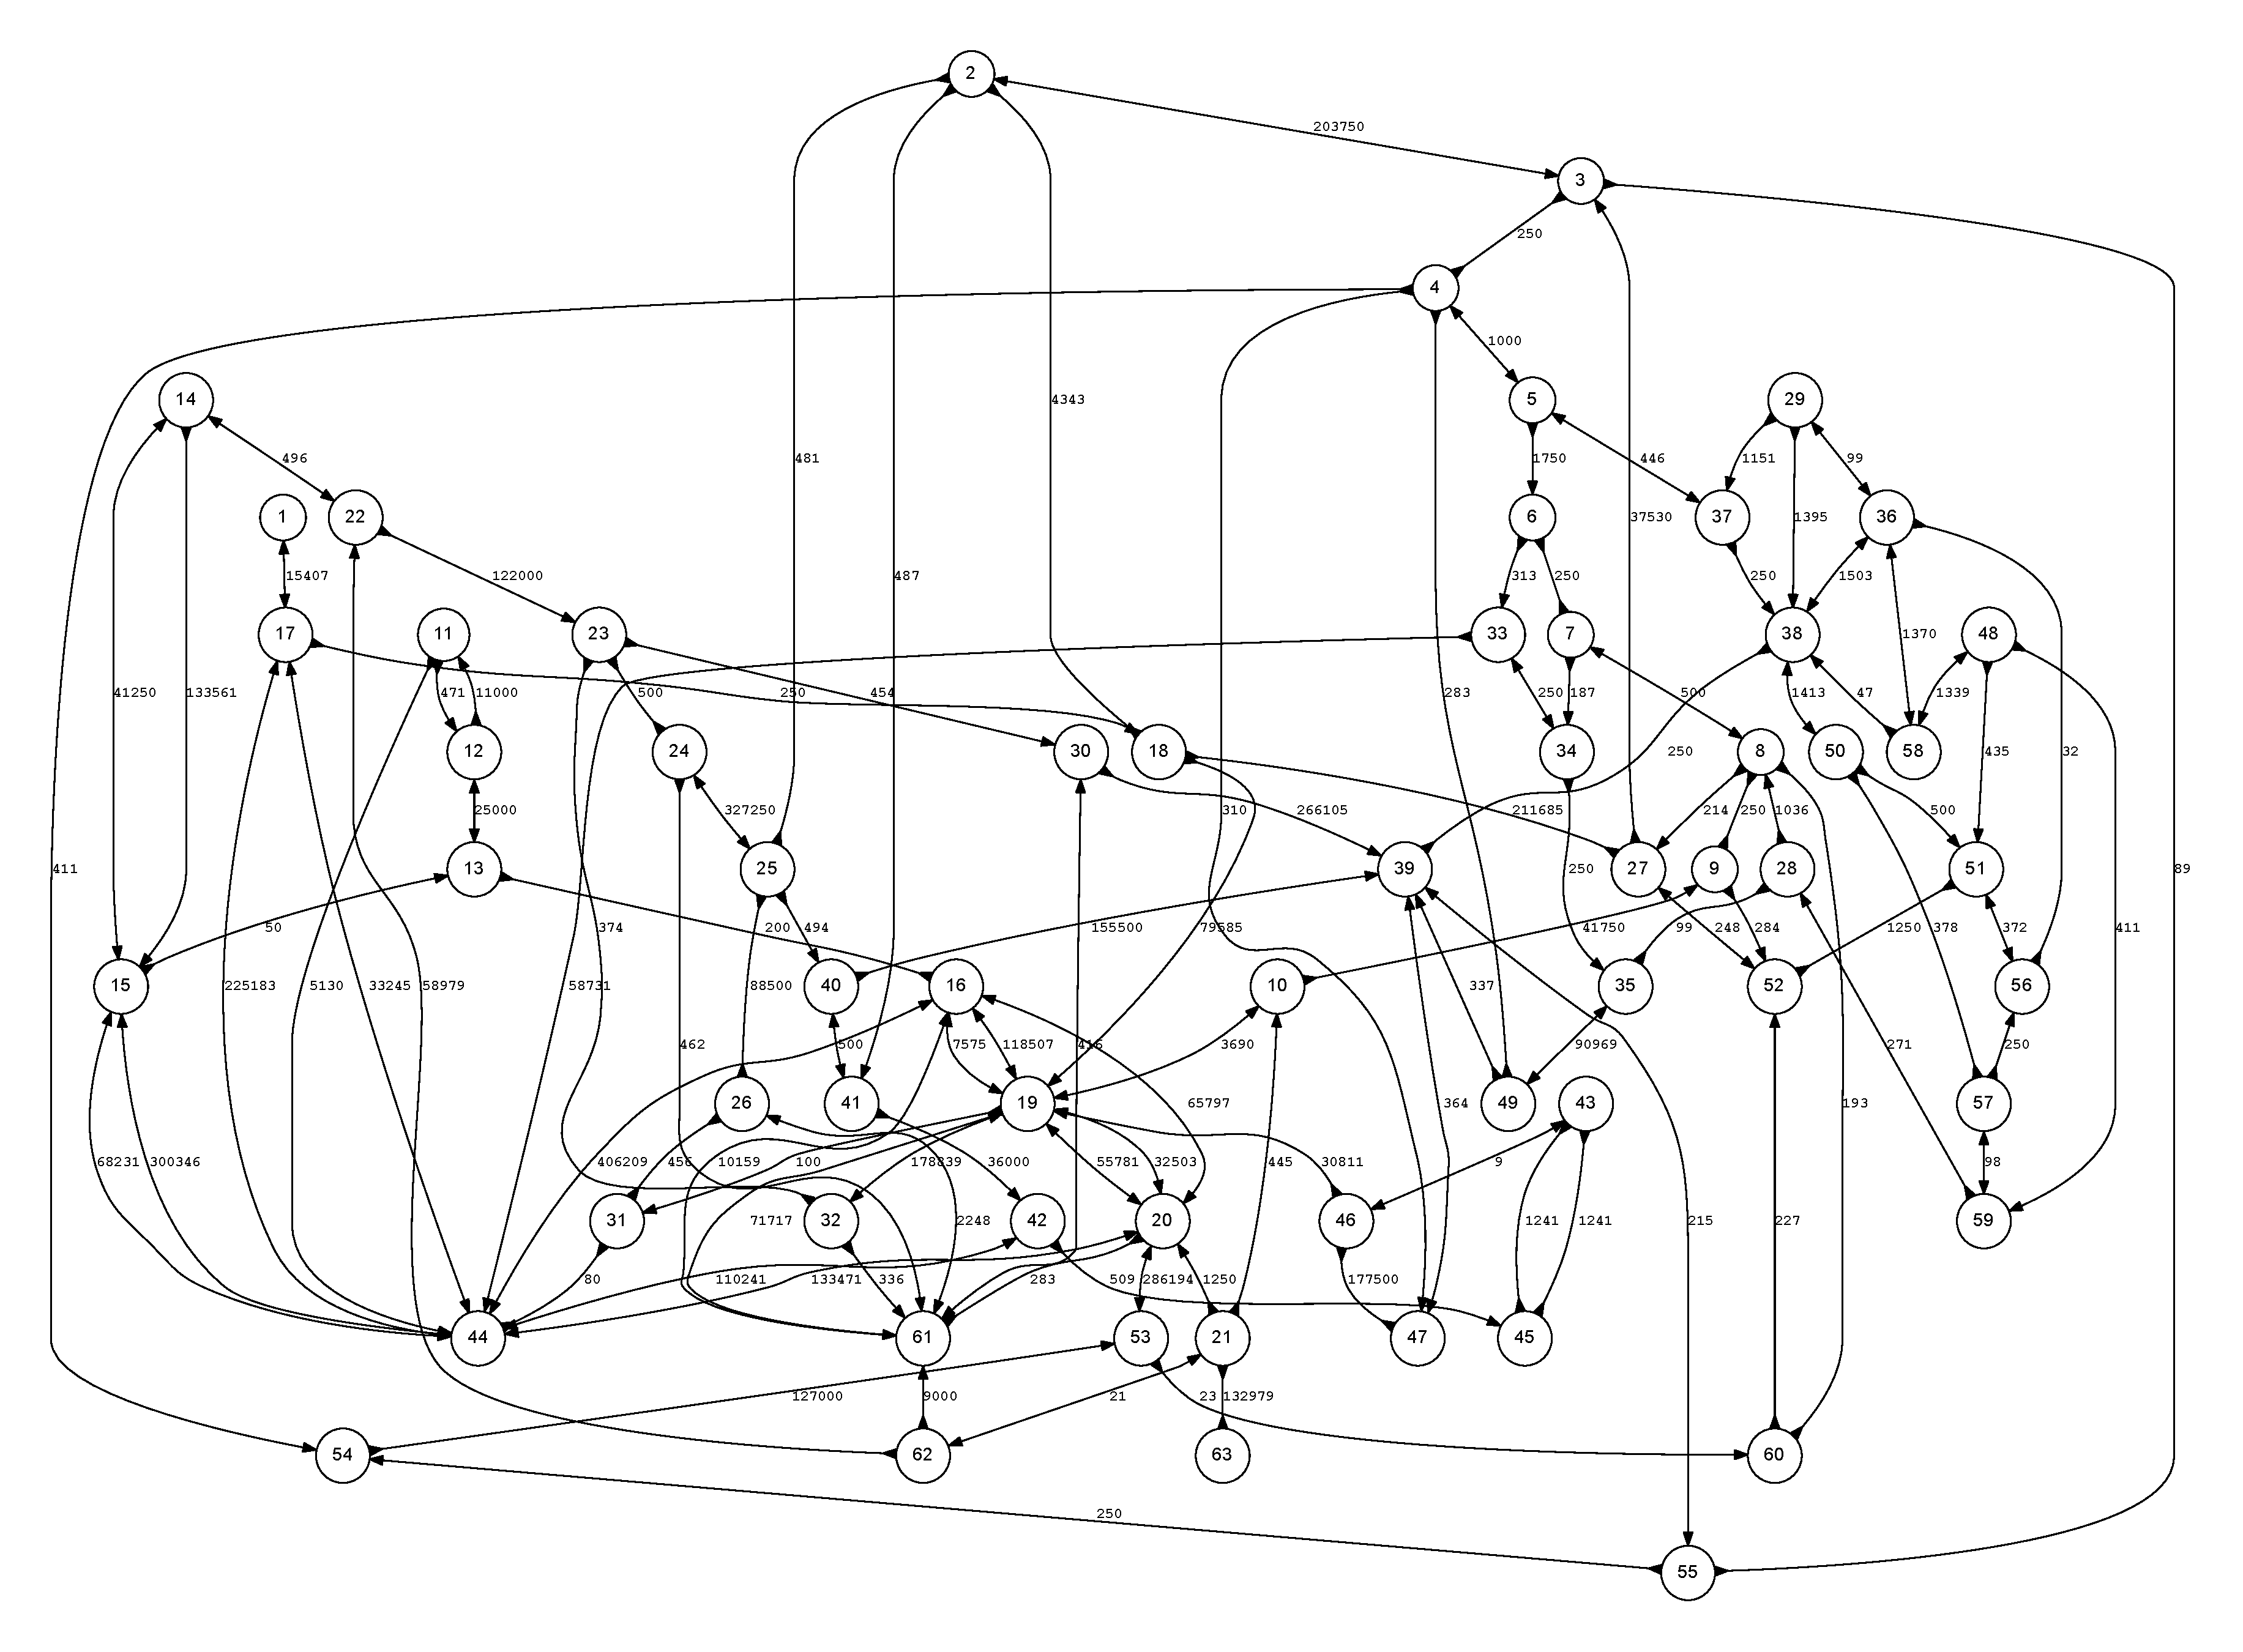
\includegraphics[width=0.6\textwidth]{E_coli.pdf}
	\end{center}
\end{frame}


\begin{frame}{Next steps}
	\begin{itemize}
		\item Given a bidirected string graph that may, in general, have
		thousands of edges and vertices even after transitive reduction and
		collapsing unbranched paths, how can we find the most likely assembly?
		\item Solution: Identify edges that may need to be traversed more than
		once, then solve a minimum-cost network flow problem to find the minimum
		number of edges that need to be traversed multiple times in order to
		make an Eulerian path.
		\item This is also similar to the Chinese Postman Problem, but this is a
		{\it bidirected graph}, and we are also okay with the final
		reconstruction of the genome still being discontinuous, rather than a
		single path (if necessary).
	\end{itemize}
\end{frame}

\begin{frame}{Implementation}
	\begin{minipage}{0.3\textwidth}
		\begin{itemize}
			\item A set of C++ programs that iteratively transform the data into
			the final assembly.
			\item Yellow programs are not yet implemented.
		\end{itemize}
	\end{minipage}
	\begin{minipage}{0.67\textwidth}
		\includegraphics[width=1.0\textwidth]{programs.pdf}
	\end{minipage}
\end{frame}

%\begin{frame}{Effectiveness on random genomes}
	%\begin{itemize}
		%\item Error-free 250bp reads sampled from random strands of the full {\it
		%E. coli} genome (4,639,675 bp) with 100bp separation.
		%\item 46,392 reads $\to$ {\tt compute-overlaps} $\to$
	%\end{itemize}
	%\begin{figure}[H]
	%\caption{
		%Bidirected string graph built from E. coli (4,639,675 bp) with uniformly sampled
		%250bp reads with 125bp minimum overlap length.  (Graph shown after transitive
		%reduction and collapsing unbranched paths)



		%}
	%\includegraphics{E_coli_full.pdf}
	%\end{figure}
%\end{frame}

%\begin{frame}{Contained reads}
%\end{frame}


%\begin{frame}{A
%17. Implementation:

\begin{comment}

14. Traversal count calculation

Estimate the traversal count of each edge.

Ideally, every edge will be traversed exactly one time.
- But, real genomes always contain repetitive sequence, and these regions may
appear multiple times in the final assembly.
- It is also possible for there to be erroneous parts of the graph that should
  not be included in the final assembly at all.

A-statistic formula

15. Minimum cost network flow

We need to determine how many times edge must be traversed.

Remember, some edges may be repeated sequence, and they therefore may appear
multiple times in the original genome.

Given the bidirected string graph with each edge labeled as OPTIONAL, EXACTLY
ONCE, or AT LEAST ONCE, compute a minimum-cost network flow that makes the graph
Eulerian.

16. Compute an Eulerian tour of the graph to produce a reconstruction of the
original genome.

A generalized Eulerian tour through the bidirected graph will produce a possible
reconstruction of the original genome.

- General case:  The original genome cannot be reconstructed in one piece, so
  the final reconstruction must take the form of the smallest set of paths that
  traverse all the edges the required number of times.

17. Implementation:

- A set of C++ programs that iteratively transform the data into the final
  assembly.
- Different sets of stages of the algorithm may be run in order to reach the
  final assembly.

Each node is a binary program.

The arrows indicate the output from one program being used in other program.


            convert-reads

                |
                V
                ...

Reads are input in textual form, e.g. the FASTA format:

>read_1
ATATTATATAT
>read_2
GCGCGTGTGTA

Genome is output in textual form.

A _contig_

>contig_1
TTTATAGTAGTAGTTGATTAGTATAGTGATGATAGTAGTA...

- Many things still would need to be improved to make this competitive with
  other assemblers.

18. References

- The Fragment String Assembly Graph (2005) by Eugene W. Myers
    * Main algorithm I have described.

- Maximum Likelihood Genome Assembly (2009) by Paul Medvedev and Michael Brudno
    * Explanation of bidirected graphs and bidirected graph algorithms applied
    * to DNA sequences.
\end{comment}

\end{document}
